\chapter{Experimental Setup}

The second NCAL campaign at \NCALInstitute was carried out in the proton-driven neutron environment of the U-120M cyclotron. This chapter summarizes the experimental arrangement relevant for interpreting detector response: the beamline geometry, detector placement, shielding layout, and the roles of the main supporting subsystems. Detailed source-reaction physics is treated in the next chapter, while detector construction and DAQ implementation are described later.

\section{Setup geometry and detector placement}

Figure~\ref{fig:rez2-working-setup} summarizes the layout adopted for experiment~2. The schematic records the current setup logic, detector ordering, and monitoring strategy along the beam axis, while also identifying those elements that remained under optimization during preparation of the campaign.

\begin{figure}[tbp]
\centering
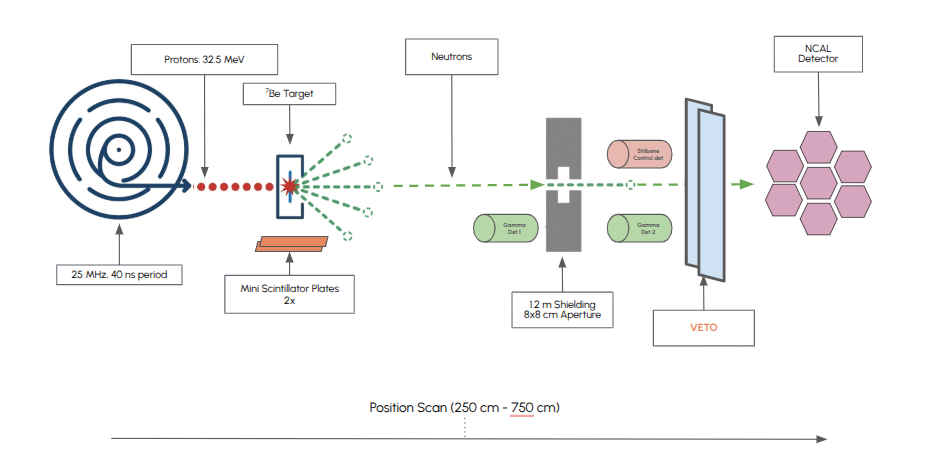
\includegraphics[width=0.98\textwidth]{figures/Experiment_Setup_rez2.png}
\caption{Schematic layout of the second experiment at \NCALInstitute. The scheme shows the proton beam delivered from the cyclotron onto a beryllium target, target-adjacent mini scintillator plates planned as a coincidence-based backup production monitor, an upstream gamma detector, a \SI{1.2}{m} shielding block with an $8 \times 8$ cm$^2$ aperture aligned to the central NCAL line of sight, a downstream gamma detector behind the shield, a compact control stilbene detector near the NCAL entrance plane, the seven-module NCAL flower geometry, and an optional thin plastic veto layer in front of the central module. The position-scan direction indicated in the sketch corresponds to the current working range of roughly \SIrange{250}{750}{cm}. Several elements, especially the target-adjacent scintillators, the exact control-detector placement, and the use of the front veto layer, remained part of the ongoing setup optimization.}
\label{fig:rez2-working-setup}
\end{figure}

The experiment was performed in the forward-directed mixed neutron--gamma field produced by cyclotron protons on a beryllium target. The forward radiation field emerging from the target was sampled downstream along the axis of the planned NCAL position scan. The drawing presently labels the proton beam with an energy of \SI{32.5}{MeV} and also marks the cyclotron RF structure as \SI{25}{MHz} with a \SI{40}{ns} period. These values are retained here as setup identifiers from the current experiment sketch and should be cross-checked against the run-time machine settings recorded during the actual campaign.

One distinctive feature of the planned geometry is the pair of mini scintillator plates placed immediately next to the target and oriented toward the production point. In the present concept they are intended to operate in coincidence mode and to provide a local indication that production is taking place near the target. Their role is explicitly secondary: they are currently treated as a backup or plan-B monitoring option rather than as a validated primary beam monitor. Their efficiency in the actual source geometry, their count-rate capability, and even their practical usefulness under the expected radiation conditions are not yet established and will need to be tested experimentally.

Farther downstream, the first gamma detector is intended to monitor the prompt and background gamma field before the main shielding block. The present expectation is that this detector may provide both gamma-spectral information and useful timing information associated with prompt gamma production. A \SI{1.2}{m} thick shielding block with an $8 \times 8$ cm$^2$ aperture is then used to define the line of sight toward the central NCAL module. In the current layout logic, the aperture is not merely a mechanical opening but part of the background-reduction strategy: it restricts the direct acceptance to the intended central region while allowing the surrounding shield to suppress off-axis radiation.

Behind this shielding block, a second gamma detector is planned upstream of NCAL but in a substantially more shielded location than the first one. Its intended role is to characterize the radiation field that survives the shielding and reaches the NCAL entrance region. In the most conservative wording, this means measuring the gamma spectrum behind the shielding; depending on detector response and local mixed-field conditions, the same detector may also record neutron-induced contributions, but that possibility should be treated as an effect to be measured rather than assumed a priori.

The control stilbene detector is presently envisaged near the NCAL entrance plane as a reference neutron monitor with known neutron-detection performance. Its exact position, however, remains an open optimization problem. From one point of view, the most direct comparison would place it on the same central line of sight as the central NCAL module. From another point of view, material placed directly in front of NCAL may partially shadow the calorimeter acceptance or generate additional secondary particles. For that reason, the final measurement sequence may need to alternate between different control-detector positions, or between control-detector and unobstructed NCAL configurations, instead of assuming a single permanent placement from the outset.

The NCAL detector itself is planned in the seven-module flower arrangement consisting of one central module surrounded by six peripheral modules in a honeycomb-like hexagonal pattern. The central module is aligned with the shielding aperture and therefore defines the primary line of interest in the present setup concept. In addition, a thin plastic scintillator layer may be placed in front of the central module as a veto for charged particles. At present this veto layer should be regarded as a diagnostic option rather than an established component of the finalized setup. The current expectation from the local beamline side is that charged particles should not emerge from the target region in a way that significantly reaches the NCAL position, but this statement still requires direct confirmation under the actual experimental conditions.

\section{Experimental subsystems and their roles}

Although the NCAL prototype is the detector under study, the full experiment involves several coupled subsystems. Their roles are summarized in Table~\ref{tab:experiment-subsystems}. This distinction is important because later chapters discuss some of these elements separately in terms of hardware documentation, but at experiment level they function together as one measurement system.

\begin{table}[htbp]
\centering
\caption{Main experimental subsystems and their role in the present campaign.}
\label{tab:experiment-subsystems}
\small
\setlength{\tabcolsep}{5pt}
\renewcommand{\arraystretch}{1.08}
\begin{tabularx}{\textwidth}{>{\raggedright\arraybackslash}p{3.5cm}YY}
\toprule
Subsystem & Role in the experiment & Main observables or function \\
\midrule
NCAL prototype & Detector under study & Neutron response, timing behavior, detector stability, and future efficiency-related observables \citep{Okropiridze2024SimulationNCAL,Okropiridze2026NCALAddendum}. \\
Target-adjacent mini scintillator pair (planned) & Backup production monitor near the target & Local coincidence signal near the production point; presently a contingency monitor whose practical efficiency is not yet established. \\
First gamma detector & Upstream mixed-field monitor & Prompt-gamma timing information and gamma-spectrum monitoring before the main shielding block. \\
Shielding block with central aperture & Passive background reduction and geometrical selection & Restricts the direct line of sight toward the central NCAL module while suppressing off-axis radiation. \\
Second gamma detector & Downstream radiation-field monitor & Characterization of the radiation field behind shielding and in front of NCAL, primarily gamma-sensitive but potentially recording mixed-field contributions. \\
Control stilbene detector & Reference neutron monitor & Relative neutron-flux monitoring close to the NCAL entrance region, with placement still under optimization. \\
Optional thin plastic veto layer & Charged-particle check at the NCAL entrance plane & Diagnostic veto option intended to test whether any charged-particle contamination reaches the calorimeter position. \\
DAQ and front-end chains & Signal transport and event building & Trigger-referenced observables such as timestamps, time-over-threshold values, timing jitter, waveform shapes, and firmware-derived quantities. \\
\bottomrule
\end{tabularx}
\end{table}

The upstream and downstream gamma detectors, the control stilbene detector, and the target-adjacent mini scintillators each probe a different part of the radiation field and together provide the contextual information needed to interpret the NCAL response. The shielding and aperture assembly likewise form an active part of the measurement definition, because they determine which fraction of the field is intentionally delivered to the calorimeter entrance.

\section{Measurement strategy}

The measurement strategy is centered on the NCAL flower geometry aligned to the shielding aperture and studied along the beam axis over the planned source-to-detector distance range indicated in Fig.~\ref{fig:rez2-working-setup}. Supporting detectors are used to characterize different components of the local radiation field: the upstream gamma detector samples the prompt field before shielding, the downstream gamma detector characterizes the radiation that reaches the NCAL entrance region, and the control stilbene detector provides a neutron-sensitive reference close to the calorimeter position.

Additional configuration changes remain part of the experimental strategy where required by the measurement conditions. In particular, the exact placement of the control stilbene detector may be alternated to avoid permanent shadowing of the central NCAL line of sight, and the thin plastic veto layer may be inserted as a diagnostic configuration to test for any charged-particle contribution at the calorimeter entrance. Within this framework, the later analysis can focus on direct NCAL observables together with the contextual timing and background information delivered by the supporting detector chains.